\documentclass[10pt]{beamer}
\usetheme{Boadilla}
\usecolortheme[named=black]{structure}
\setbeamercolor{normal text}{fg=black,bg=white}
\setbeamercolor{alerted text}{fg=black}

\usepackage[utf8]{inputenc}
\usepackage{amsmath,amssymb}
\usepackage{tikz}
\usetikzlibrary{positioning}

% ---------- Footer: page number (left) + department name (right) ----------
\setbeamertemplate{footline}{%
  \leavevmode%
  \hbox{%
  \begin{beamercolorbox}[wd=.5\paperwidth,ht=2.5ex,dp=1.125ex,left,leftskip=1em]{author in head/foot}%
    \usebeamerfont{author in head/foot}\insertframenumber{} / \inserttotalframenumber
  \end{beamercolorbox}%
  \begin{beamercolorbox}[wd=.5\paperwidth,ht=2.5ex,dp=1.125ex,right,rightskip=1em]{title in head/foot}%
    \usebeamerfont{title in head/foot}Dept. of CSE (AI \& SE)
  \end{beamercolorbox}}%
  \vskip0pt%
}
\setbeamertemplate{navigation symbols}{}

\title{Mathematics for Computing}
\subtitle{Assignment}
\author{Aleena Mary John}
\institute{Department of Computer Science and Engineering \\ with Artificial Intelligence and Software Engineering}
\date{\today}

\begin{document}

% ---------------- Title Page ----------------
\begin{frame}
  \titlepage
\end{frame}

% ---------------- Outline ----------------
\begin{frame}{Outline}
  \tableofcontents
\end{frame}

% ================================================================
\section{Sets}
\begin{frame}{Sets}
  \begin{itemize}
    \item A \textbf{set} is a well-defined collection of distinct objects, called \textbf{elements} or \textbf{members}.
    \item Sets are usually denoted by capital letters ($A, B, C, \dots$) and elements by lowercase letters.
    \item Membership is written as $x \in A$ ($x$ belongs to $A$) or $x \notin A$ ($x$ does not belong to $A$).
    \item A set can be represented in two main ways:
    \begin{itemize}
      \item \textbf{Roster (Tabular) Form:} listing all elements, e.g. $A = \{1,2,3,4,5\}$
      \item \textbf{Set Builder (Rule) Form:} describing a property satisfied by the elements
    \end{itemize}
  \end{itemize}
\end{frame}

% ================================================================
\section{Set Builder Form}
\begin{frame}{Set Builder Form}
  \begin{itemize}
    \item In set builder form, a set is written as:
    \[
      A = \{\, x \mid P(x) \,\}
    \]
    read as ``$A$ is the set of all $x$ such that $x$ satisfies property $P$''.
    \item It is useful when listing all elements is impossible or impractical (e.g. infinite sets).
  \end{itemize}
\end{frame}

\begin{frame}{Set Builder Form --- 10 Examples (1/2)}
  \small
  \begin{enumerate}
    \item $A = \{ x \mid x \in \mathbb{N},\ x < 10 \} = \{0,1,2,3,4,5,6,7,8,9\}$
    \item $B = \{ x \mid x \in \mathbb{Z},\ x^2 = 4 \} = \{-2, 2\}$
    \item $C = \{ x \mid x \text{ is a vowel in the English alphabet} \} = \{a,e,i,o,u\}$
    \item $D = \{ x \mid x \in \mathbb{R},\ 0 \le x \le 1 \}$ \quad (the closed interval $[0,1]$)
    \item $E = \{ x \mid x \in \mathbb{N},\ x \text{ is even},\ x \le 20 \}$
  \end{enumerate}
\end{frame}

\begin{frame}{Set Builder Form --- 10 Examples (2/2)}
  \small
  \begin{enumerate}
    \setcounter{enumi}{5}
    \item $F = \{ x \mid x \in \mathbb{N},\ x \text{ is prime},\ x < 30 \}$
    \item $G = \{ x \mid x \in \mathbb{N},\ x = n^2 \text{ for some } n \in \mathbb{N},\ x < 100 \}$
    \item $H = \{ x \mid x = 2n,\ n \in \mathbb{N} \}$ \quad (all positive multiples of 2)
    \item $I = \{ x \mid x \text{ is a day of the week starting with the letter } S \} = \{\text{Saturday, Sunday}\}$
    \item $J = \{ (x,y) \mid x, y \in \mathbb{R},\ x^2 + y^2 = 1 \}$ \quad (points on the unit circle)
  \end{enumerate}
\end{frame}

% ================================================================
\section{Types of Sets}
\begin{frame}{Types of Sets --- AI/DS Examples (1/2)}
  \scriptsize
  \begin{itemize}
    \item \textbf{Empty (Null) Set} $\emptyset$: has no elements.
    \\ E.g. $\{x \mid x \text{ is a test sample with negative age}\} = \emptyset$
    \item \textbf{Singleton Set}: exactly one element.
    \\ E.g. $\{\text{accuracy}\}$ --- a model evaluated using a single metric
    \item \textbf{Finite Set}: countable number of elements.
    \\ E.g. $\{\text{cat, dog, bird}\}$ --- class labels in a classification problem
    \item \textbf{Infinite Set}: unending number of elements.
    \\ E.g. the set of all possible real-valued weights in a neural network layer
    \item \textbf{Equal Sets} ($A = B$): same elements, regardless of order.
    \\ E.g. the set of unique tokens in two identical text documents
    \item \textbf{Equivalent Sets} ($A \sim B$): same cardinality, not necessarily same elements.
    \\ E.g. $\{5 \text{ input features}\} \sim \{5 \text{ hyperparameters}\}$
  \end{itemize}
\end{frame}

\begin{frame}{Types of Sets --- AI/DS Examples (2/2)}
  \scriptsize
  \begin{itemize}
    \item \textbf{Subset} ($A \subseteq B$): every element of $A$ is in $B$.
    \\ E.g. selected features $\subseteq$ all available features
    \item \textbf{Proper Subset} ($A \subset B$): $A \subseteq B$ and $A \neq B$.
    \\ E.g. training set $\subset$ full dataset
    \item \textbf{Universal Set} $U$: the set containing all objects under consideration.
    \\ E.g. $U = \{0,1,\dots,255\}$ --- all possible pixel intensities in an 8-bit image
    \item \textbf{Power Set} $\mathcal{P}(A)$: the set of all subsets of $A$; $|\mathcal{P}(A)| = 2^{|A|}$.
    \\ E.g. $\mathcal{P}(\text{feature set})$ --- all possible feature subsets tried during feature selection
    \item \textbf{Disjoint Sets} ($A \cap B = \emptyset$): sets with no common elements.
    \\ E.g. the training set and the test set are disjoint (no overlapping samples)
  \end{itemize}
\end{frame}

% ================================================================
\section{Set Operations}
\begin{frame}{Set Operations --- Definitions and a Simple Example}
  \small
  Let $A = \{1,2,3\}$, $B = \{2,3,4\}$, and universal set $U = \{1,2,3,4,5\}$.
  \begin{itemize}
    \item \textbf{Union:} $A \cup B = \{x \mid x \in A \text{ or } x \in B\} = \{1,2,3,4\}$
    \item \textbf{Intersection:} $A \cap B = \{x \mid x \in A \text{ and } x \in B\} = \{2,3\}$
    \item \textbf{Difference:} $A - B = \{x \mid x \in A \text{ and } x \notin B\} = \{1\}$
    \item \textbf{Complement:} $A' = \{x \mid x \in U \text{ and } x \notin A\} = \{4,5\}$
    \item \textbf{Symmetric Difference:} $A \triangle B = (A - B) \cup (B - A) = \{1,4\}$
  \end{itemize}
\end{frame}

% ================================================================
\section{Inclusion--Exclusion Principle}
\begin{frame}{Inclusion--Exclusion Principle --- Three Sets}
  \[
    |A \cup B \cup C| = |A|+|B|+|C| - |A\cap B| - |B\cap C| - |A\cap C| + |A\cap B\cap C|
  \]
\end{frame}

\begin{frame}{Inclusion--Exclusion Principle --- General ($n$ Sets)}
  \[
    \left| \bigcup_{i=1}^{n} A_i \right|
    = \sum_{i=1}^{n} |A_i|
    - \sum_{i<j} |A_i \cap A_j|
    + \sum_{i<j<k} |A_i \cap A_j \cap A_k|
    - \cdots
    + (-1)^{n+1} \left| \bigcap_{i=1}^{n} A_i \right|
  \]
\end{frame}

% ================================================================
\section{Hasse Diagrams}
\begin{frame}{Hasse Diagrams}
  \small
  \begin{itemize}
    \item A \textbf{Hasse diagram} is a graphical representation of a finite \textbf{partially ordered set (poset)}.
    \item Rules for drawing:
    \begin{itemize}
      \item Loops (self-relations) are omitted.
      \item Edges implied by transitivity are omitted.
      \item If $a \prec b$ ($a$ is related to $b$, $a \neq b$), $b$ is drawn \textbf{above} $a$, connected by a line (no arrowhead needed).
    \end{itemize}
    \item Commonly used to represent divisibility, subset relations, etc.
  \end{itemize}
\end{frame}

\begin{frame}{Hasse Diagram --- Example}
  \centering
  Divisibility relation on $A = \{1,2,3,4,6,12\}$
  \vspace{0.3cm}

  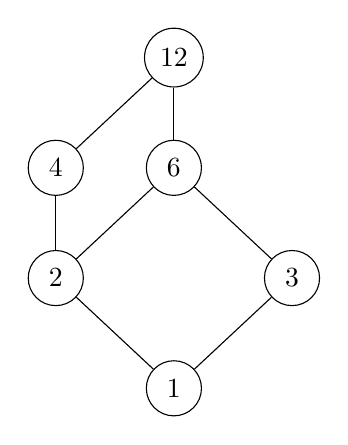
\begin{tikzpicture}[node distance=1.4cm, every node/.style={circle, draw, minimum size=0.7cm}]
    \node (n1) at (0,0) {1};
    \node (n2) at (-1.5,1.4) {2};
    \node (n3) at (1.5,1.4) {3};
    \node (n4) at (-1.5,2.8) {4};
    \node (n6) at (0,2.8) {6};
    \node (n12) at (0,4.2) {12};

    \draw (n1) -- (n2);
    \draw (n1) -- (n3);
    \draw (n2) -- (n4);
    \draw (n2) -- (n6);
    \draw (n3) -- (n6);
    \draw (n4) -- (n12);
    \draw (n6) -- (n12);
  \end{tikzpicture}

  \vspace{0.3cm}
  \footnotesize $a \prec b$ here means $a$ divides $b$. Note that the edge $1$--$12$ is omitted since it follows by transitivity.
\end{frame}

\begin{frame}
  \centering
  \Large Thank You
\end{frame}

\end{document}